\documentclass{article}
\usepackage[margin=0.75in]{geometry}
\usepackage{amsmath}
\usepackage{physics}
\usepackage{listings}
\usepackage{caption}
\usepackage{graphicx}
\usepackage{algorithm}
\usepackage{algpseudocode}
\usepackage{setspace} \doublespacing
\graphicspath{{../Images/}}


\title{PHYS 471 Research Plan: Autocatalytic Reaction Networks}
\author{Varun Varanasi}
\begin{document}


\maketitle

My proposed project for PHYS 471 is an investigation of autocatalytic reaction networks under the guidance of Professor Jun Korenaga.
This project is the continuation of a two semester senior thesis for my degree in Intensive Physics. The scope of this project lies under the large umbrella of theoretical biology studying the origin of life. 

In particular, my project is focused on studying the structure and dynamics of autocatalytic reaction networks. These reaction networks are defined by their ability to produce species that catalyze other steps within the reaction network. In our contemporary understanding of abiogenesis, the origin of life, autocatalysis and self-replication are necessary steps in the evolution of complex and interlinked biological systems. Recent advances in autocatalytic reaction theory have developed an algorithm to identify RAF reaction networks. This subtype of reaction networks can be understood as the barebones of an autocatalytic reaction network in which each reaction is catalyzed by a product of another reaction in the reaction set. Furthermore, each product produced in the network is a function of the action of a series of reactions on an initial food set (starting materials). Despite these models remaining our best understanding of autocatalytic reaction networks, they remain highly idealized. 

The goal of this project is broadly to test the robustness of the RAF model.
My work last semester was focused on studying the defining characteristics of these sets.
In particular, my work focused on mapping network properties and graph characteristics to the presence of autocaralytic sets. 
Additionally, I investigated the stability and robustness of autocatalytic sets in existing models to random catalytic perturbations. 
This semester I plan on expanding my past work by relaxing the idealism in the existing model. 
In particular, I am fascinated in study the temporal dynamics of these networks. 
I would like to investigate how these networks establish and evolve over time as a function of rates of reaction.
While this is a broadly phrased question, I am generally hoping to see if this additional complexity will introduce new stable states in the RAF space. 

\begin{figure}[H]
    \centering
    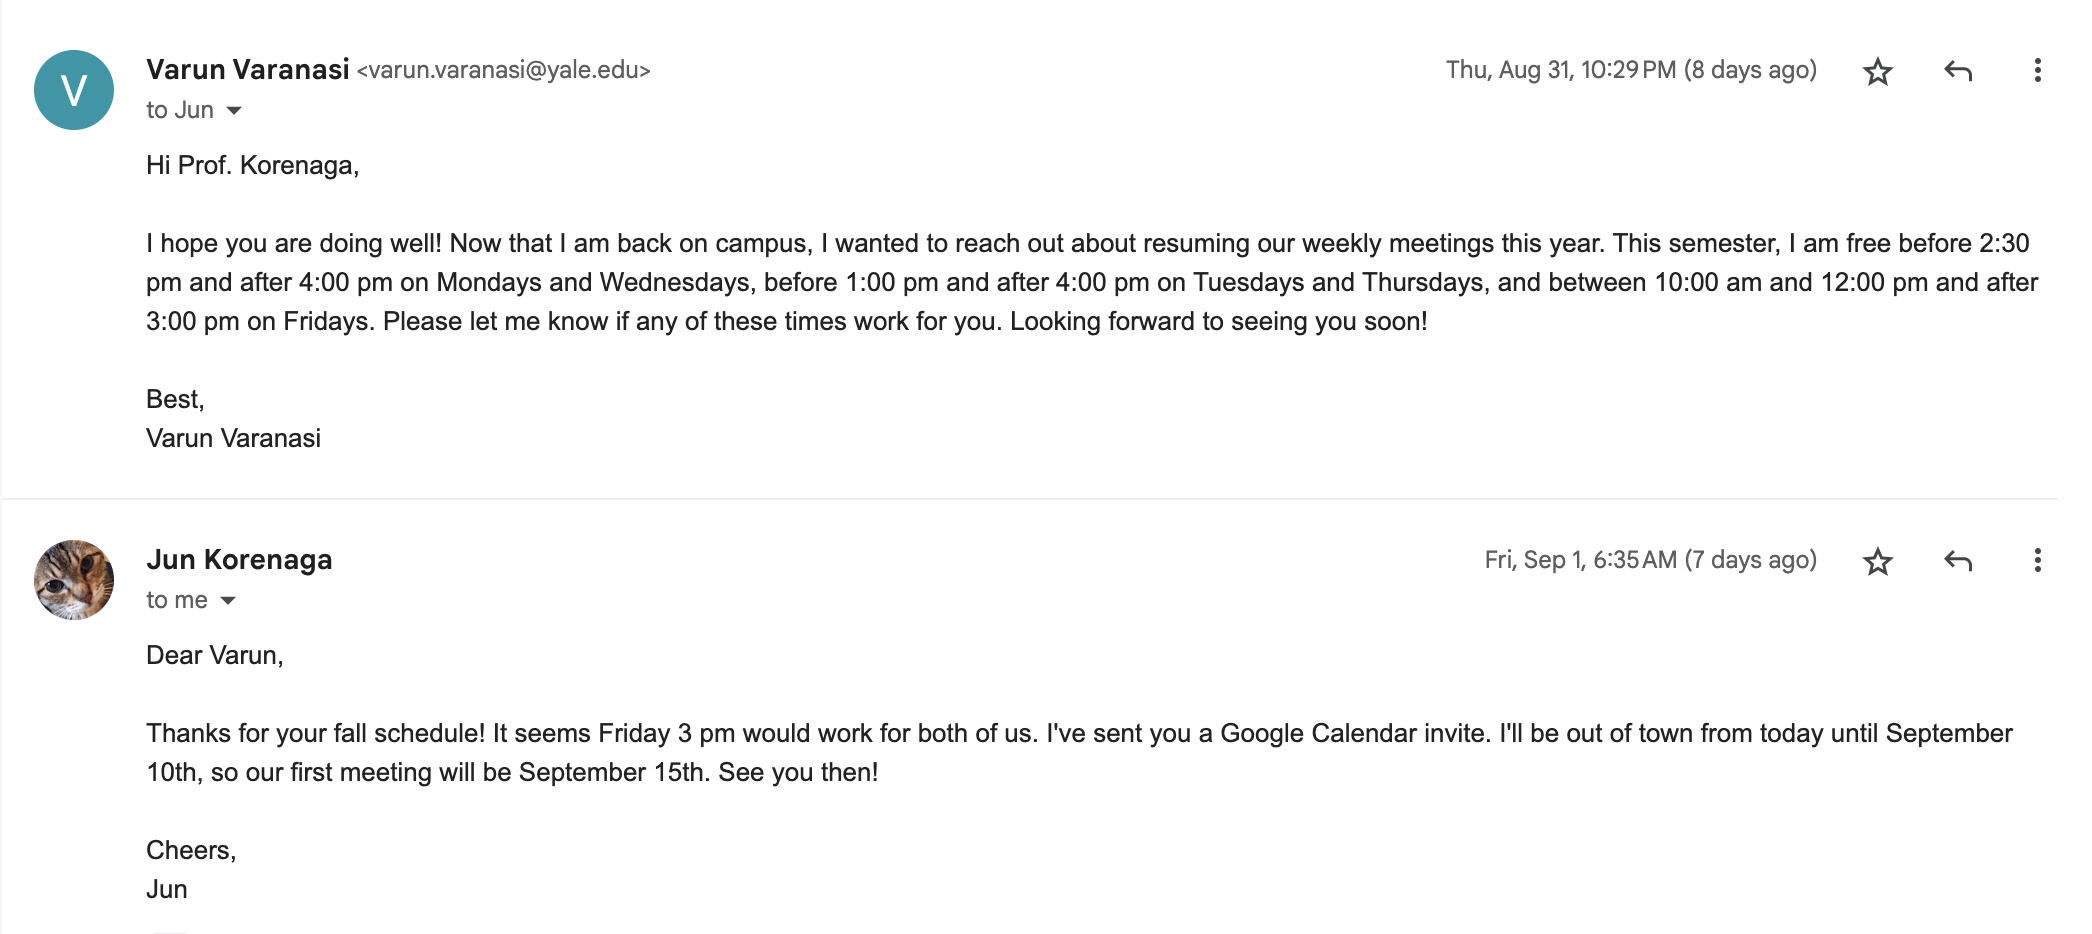
\includegraphics[width=15cm]{confirmation}
    \caption{Confirmation Email}
\end{figure}

\end{document}